\section{Video-LDM}
\label{sec:videoldm}

Video-LDM (2023) by NVIDIA \cite{video_ldm} is a T2V model based on LDM. It first trains an image generator on image datasets, then freeze the layers, and then adds temporal layers which helps to align images in temporally consistent manner, transforming it from T2I model to T2V model. Then the model is fine-tuned on video dataset. Freezing the spatial layers transforms the image generation knowledge to the video domain. The model achieves high resolutions of up to $1280\times 2048$.


\subsection*{Mathematical notations}

The LDMs AE compresses the high-dimensional input data $x \in \mathbb{R}^{T \times 3 \times \hat{H} \times \hat{W}}$ where $x \sim p_{\text{data}}$ is a sequence of $T$ RGB frames with height $\hat{H}$ and width $\hat{W}$ to lower-dimensional latent space $z = \mathcal{E} (x) \in \mathbb{R}^{T \times C \times H \times W}$ (where $C$ is the number of latent channels, and $H, W$ are the spatial latent dimensions). The model then learns to reconstruct $x$ with the decoder $\mathcal{D}$: $\hat{x} = \mathcal{D} (\mathcal{E} (x)) \sim x$.

Let us denote the spatial layers $l^i_{\theta}$ where $\theta$ are the model's parameters, and $i$ is the layer index. We then denote the addition of temporal layers as $l^i_{\phi}$ to learn to align individual frames in a temporally consistent manner. We denote $f_{\theta, \phi}$ as the full model (with spatial and temporal layers).








\subsection{Architecture}

\begin{figure}
    \centering
    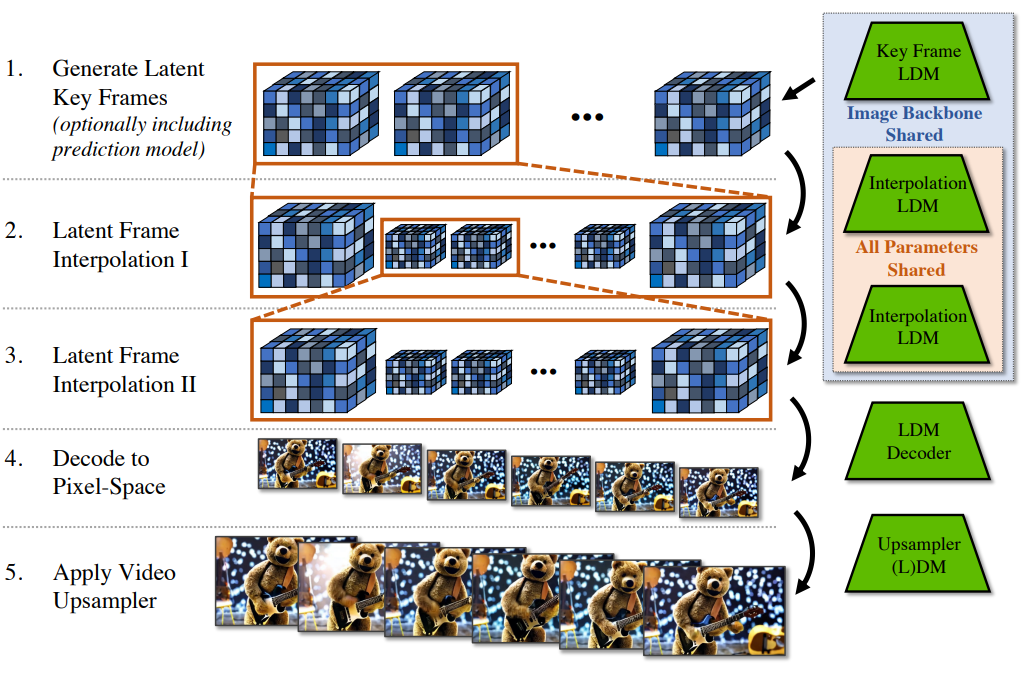
\includegraphics[width=0.7\textwidth]{images/video_ldm/stack.png}
    \caption{Video-LDM stack \cite{video_ldm}. (1) Keyframe generation. (2) Keyframe filling (keyframe interpolation). (3) Keyframe interpolation is repeated a second time. (4) The latents are decoded to pixel space. (5) Optionally, SR model is applied \cite{video_ldm}.}
    \label{fig:video_ldm_stack}
\end{figure}

The architecture of Video-LDM is similar to Stable Diffusion except for the added temporal layers, and the addition of AE for latent encoding/decoding and the discriminator which helps photorealism in the decoder network. The model's stack is shown in figure \ref{fig:video_ldm_stack}.

\begin{figure}
    \centering
    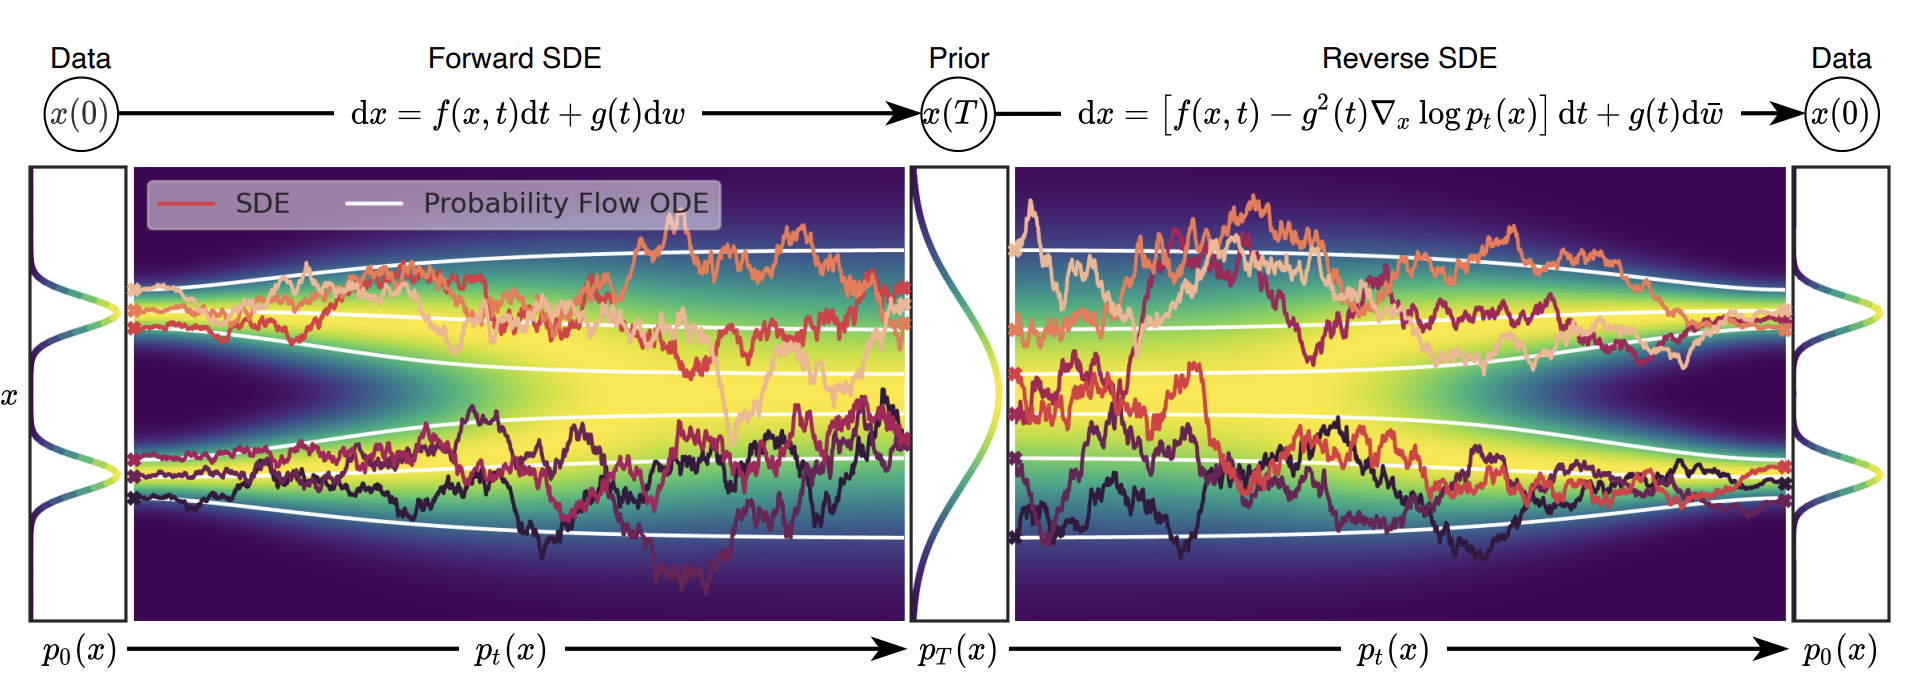
\includegraphics[width=0.6\textwidth]{images/video_ldm/ddpm_sde.png}
    \caption{Generative modeling through stochastic differential equations (SDE) \cite{song2020score}.}
    \label{fig:video_ldm_ode}
\end{figure}

Figure \ref{fig:video_ldm_ode} illustrates the stochastic diffusion process, showing SDE paths that represent sample trajectories. Data distribution $p(x)$ transitions to prior distribution $p_T(x)$ via forward SDE (adding noise) and reverses back to $p(x)$ using reverse SDE. As noise is added, structured data becomes progressively chaotic, converging to a Gaussian prior before reverting to the original distribution. The distribution depicts the data probability, the middle distribution depicts the Gaussian prior, and the right distributions depicts reconstructed data.

\begin{figure}
    \centering
    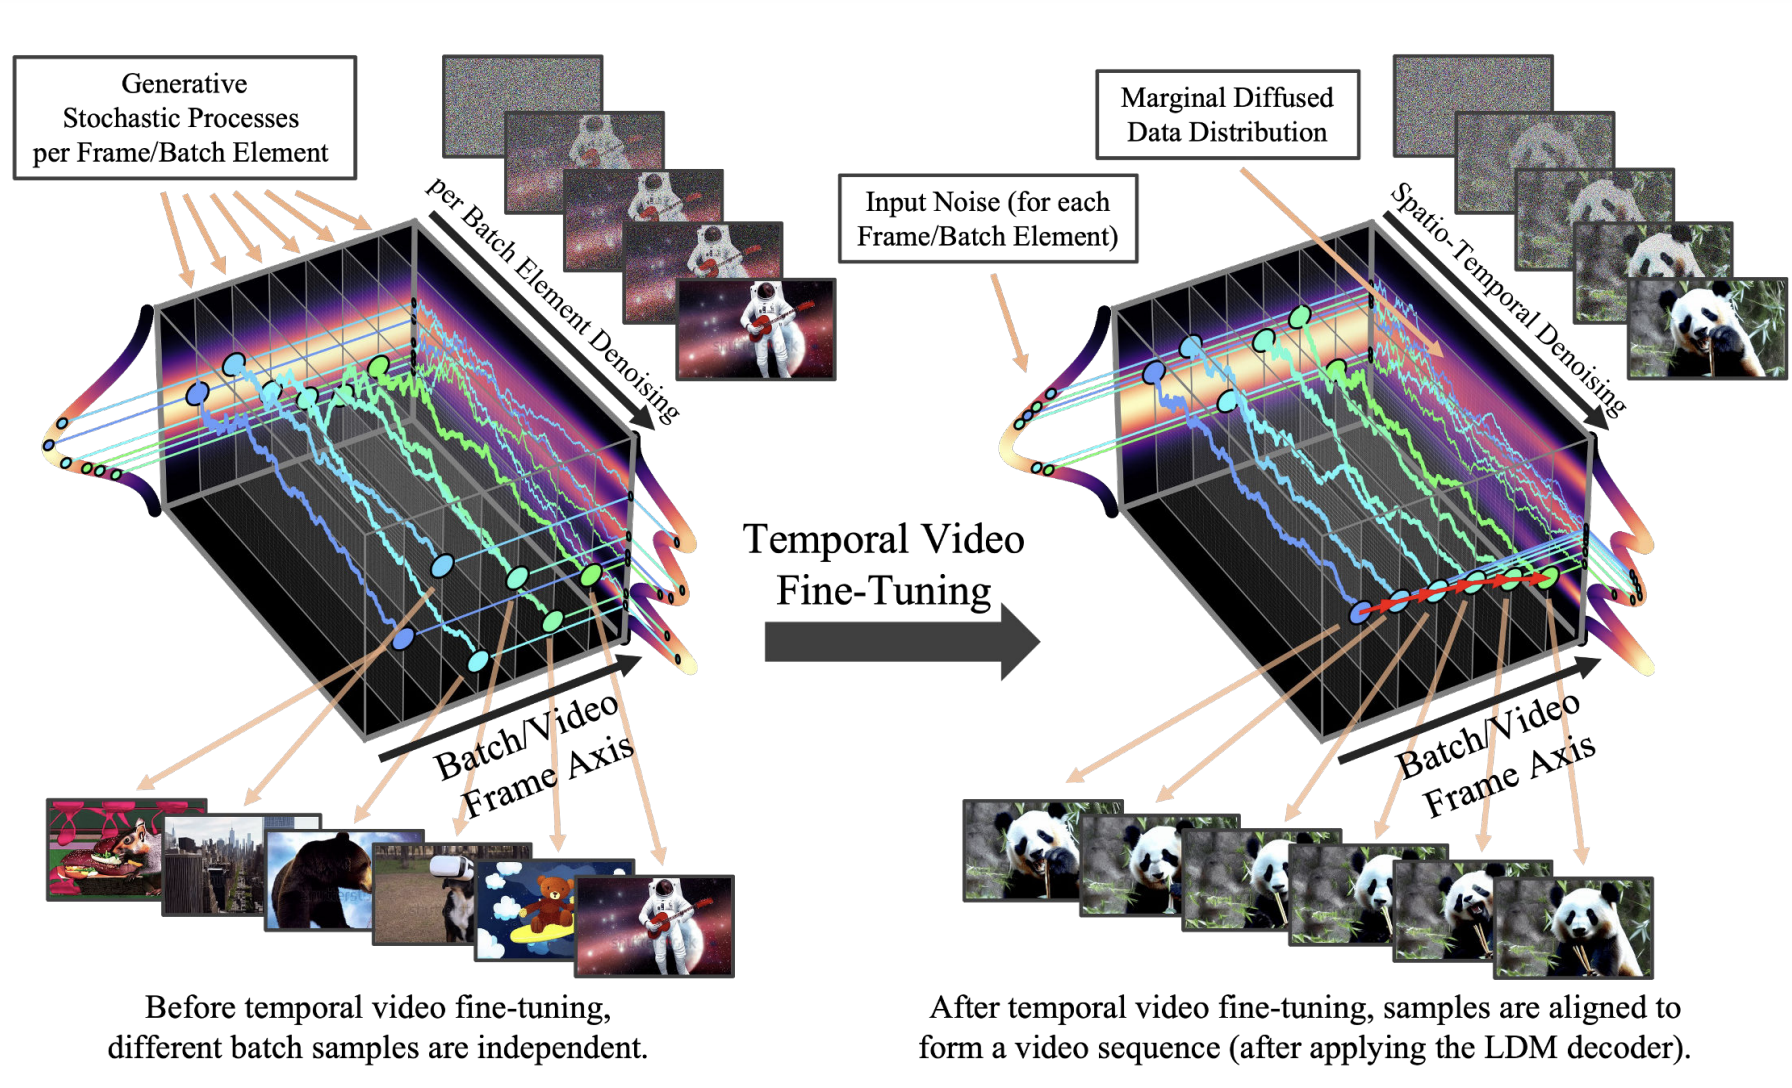
\includegraphics[width=0.8\textwidth]{images/video_ldm/image_to_video_tuning.png}
    \caption{Transforming image LDM (left) to video LDM (right) via temporal fine-tuning \cite{video_ldm}.}
    \label{fig:video_ldm_image_to_video_tuning}
\end{figure}

In figure \ref{fig:video_ldm_image_to_video_tuning} we see the temporal fine-tuning. We see the stochastic denoising process of diffusion, similar to figure \ref{fig:video_ldm_ode}. We can see that the images on the left side are not temporally aligned, whereas on the right, the images form a coherent video.

\begin{figure}
    \centering
    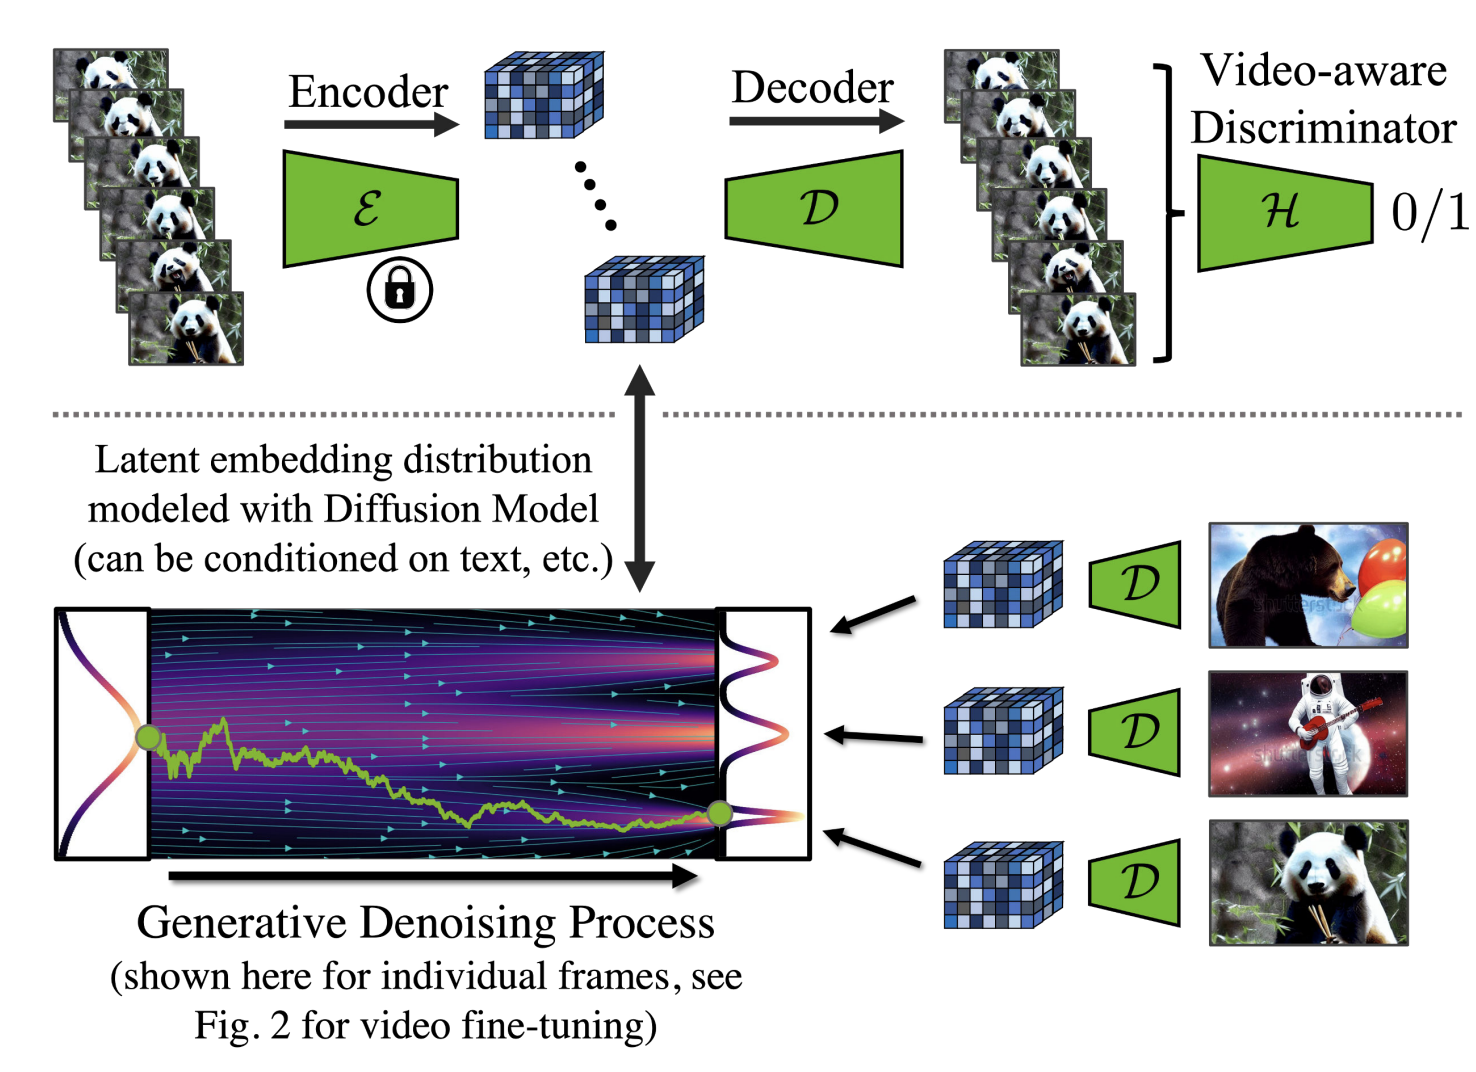
\includegraphics[width=0.6\textwidth]{images/video_ldm/enc_dec_denoise_process.png}
    \caption{\textit{Top}: frozen encoder \textit{Right}:  \textit{Bottom}: generative denoising process. \cite{video_ldm}}
    \label{fig:video_ldm_enc_dec_denoise_process}
\end{figure}

In figure \ref{fig:video_ldm_enc_dec_denoise_process} we can see the frozen encoder compresses video frames into 3D latents and the decoder learns to reconstruct them. On the right, we can see the patch-based discriminator $\mathcal{H}$ which is used to increase photorealism of the decoder. It is trained on the adversarial objective which is added to the AE reconstruction score like in PatchGAN \cite{isola2017image} (which tries to classify if $N \times N$ patch is real or fake). On the bottom we can see the generative denoising process, where each embedding corresponds to different image latent in the decoder $\mathcal{D}$.

\begin{figure}
    \centering
    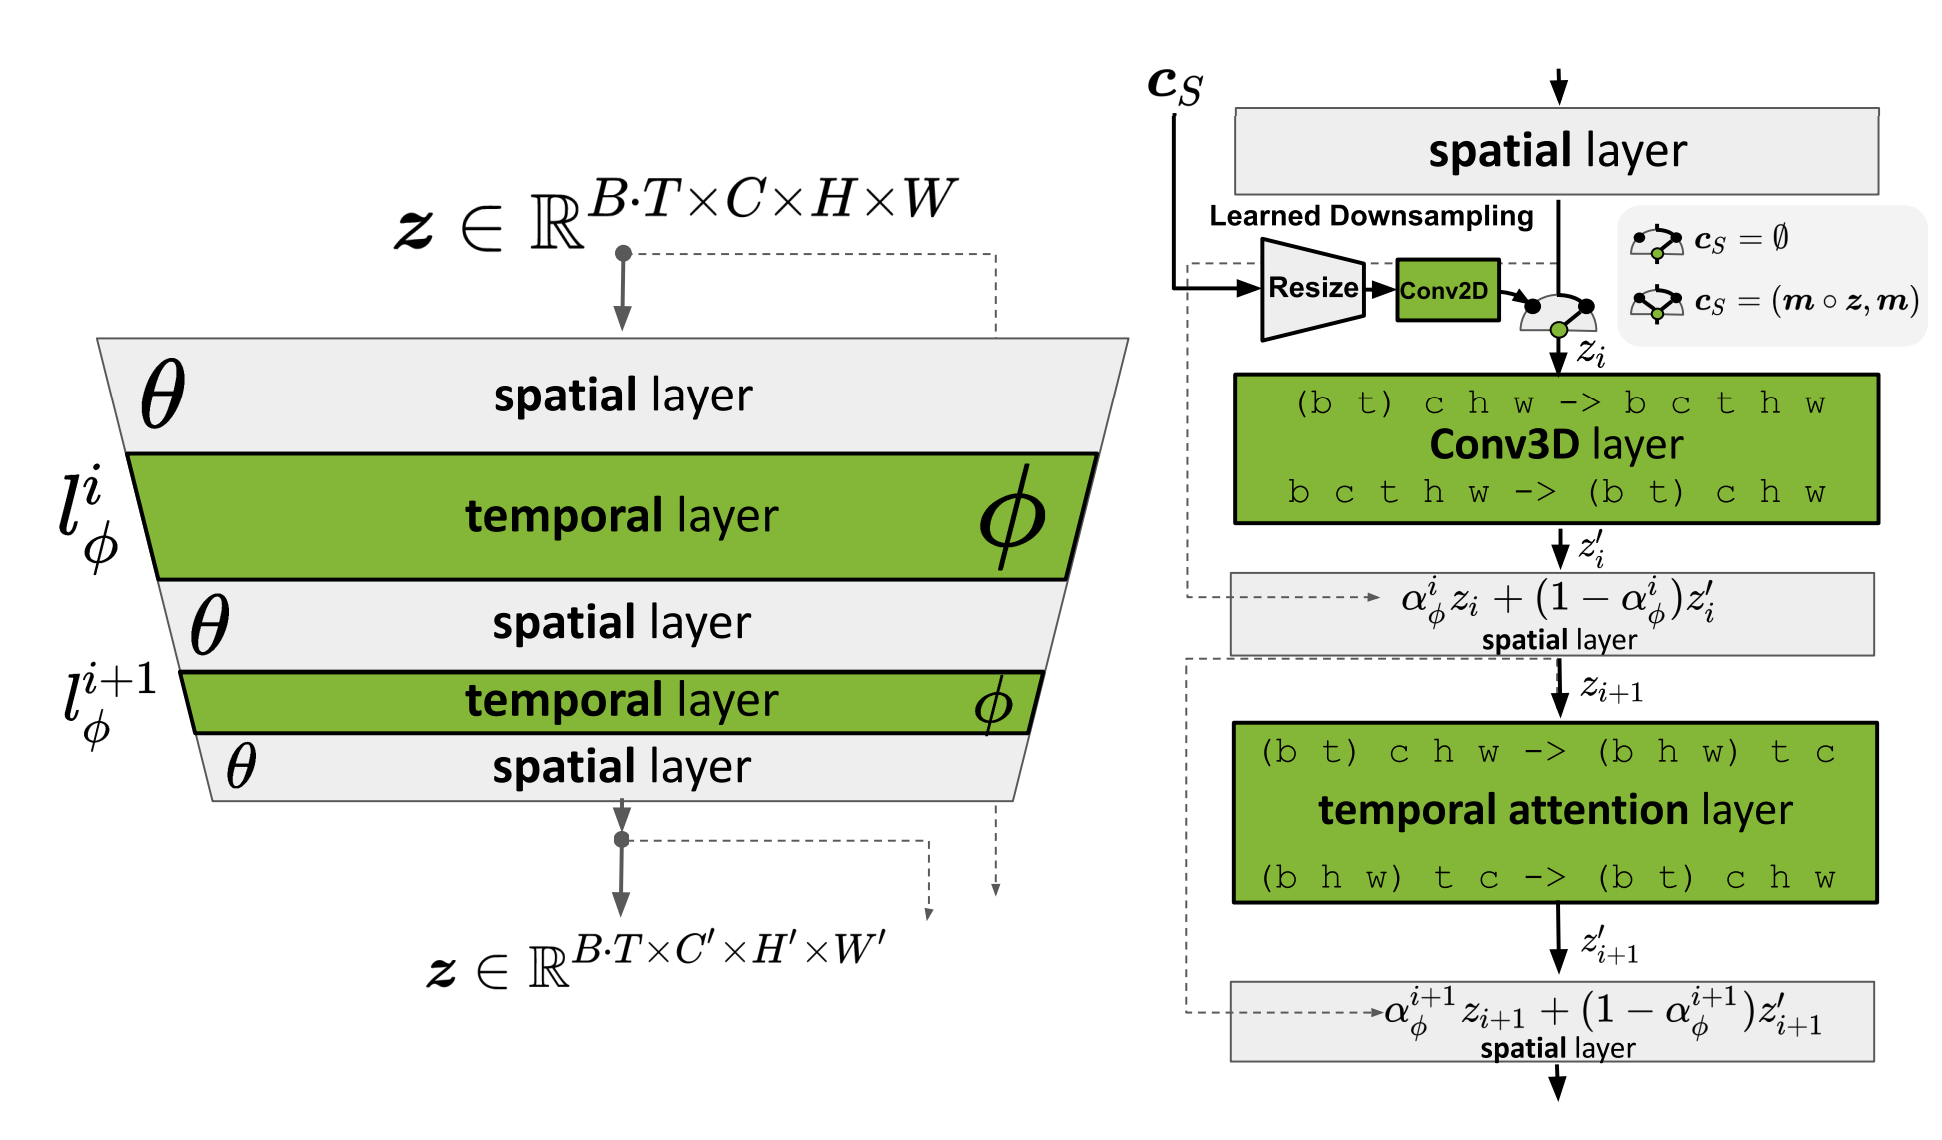
\includegraphics[width=0.6\textwidth]{images/video_ldm/temporal_layers.png}
    \caption{The researchers turn pre-trained LDM into video generator by adding temporal layers \cite{video_ldm}.}
    \label{fig:video_ldm_spatial_temporal_mixing_layers}
\end{figure}

In figure \ref{fig:video_ldm_spatial_temporal_mixing_layers} we can see on the pre-trained LDM is turned into a video generator (on the right) by adding temporal layers $l_\phi$ that learn to align images in a temporally consistent manner. The spatial layers $l_\theta$ are frozen and only the temporal layers are learned. On the right we can see closer look of spatial, temporal layers. In order to deal with the addition of the temporal dimension, they \textbf{rearranged the batch dimension} in LDM to be mixed with the temporal dimension for the next layer: $(b\ t)\ c\ h\ w \rightarrow b\ t\ c\ h\ w$. The $c_S$ represents a context vector used for conditioning the model.

The input of the spatial layers $l_\theta^i$ is of the dimension $b\ c\ h\ w$ whereas the input dimension of temporal layers is of the dimension $b\ t\ c\ h\ w$. This notation is called \texttt{Einops} (einstein operations) and is further discussed in the Einops paper \cite{einops}. The spatial layers interpret the video as a batch of images by shifting the temporal axis into the batch dimension (the spatial layers treat all $B \cdot T$ encoded video frames in the batch dimension $b$). It is important to note that the rearrange operation doesn't change the tensor values; rather it rearranges the dimensions.

For the 3D convolution (temporal layer), they reshape the input back to video dimensions (they process entire videos in new temporal dimension $t$): 

\[ \underbrace{(b\ t)\ c\ h\ w}_{\text{Output of spatial layer}} \rightarrow \underbrace{b\ c\ t\ h\ w}_{\text{Input to the next Conv3D layer}} \]

After the temporal layers they reshape the input back to fit into the spatial layers like so:

\[ \underbrace{b\ c\ t\ h\ w}_{\text{Output of Conv3D layer}} \rightarrow \underbrace{(b\ t)\ c\ h\ w}_{\text{Input to the next spatial layer}} \]

As for the temporal attention layer (temporal layer), they reshaped the input back to work on the temporal dimension, instead of spatial:

\[ \underbrace{(b\ t)\ c\ h\ w}_{\text{Output of spatial layer}} \rightarrow \underbrace{(b\ h\ w) \ t\ c}_{\text{Input to the next temporal attention layer}} \]

\[ \underbrace{(b\ h\ w) \ t\ c}_{\text{Output of temporal attention layer}} \rightarrow \underbrace{(b\ t)\ c\ h\ w}_{\text{Input to the next spatial layer}} \]

\begin{figure}
    \centering

    \begin{subfigure}{0.3\textwidth}
        \centering
        \scalebox{0.5}{
            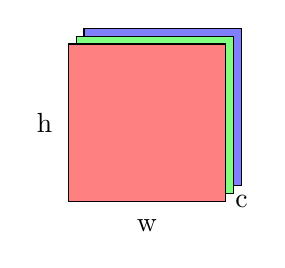
\begin{tikzpicture}
    % Blue channel slice
    \draw[fill=blue!50] (0, 0) rectangle (2, 2);

    % Green channel slice
    \draw[fill=green!50] (-0.1, -0.1) rectangle (1.9, 1.9);
    
    % Red channel slice
    \draw[fill=red!50] (-0.2, -0.2) rectangle (1.8, 1.8);

    \node at (0.8, -0.5) {w};
    \node at (-0.5, 0.8) {h};
    \node at (2, -0.2) {c};
    
\end{tikzpicture}

        }
        \caption{A single frame. The $c\ h\ w$ dimensions.}
    \end{subfigure}

    \begin{subfigure}{0.3\textwidth}
        \centering
        \scalebox{0.5}{
            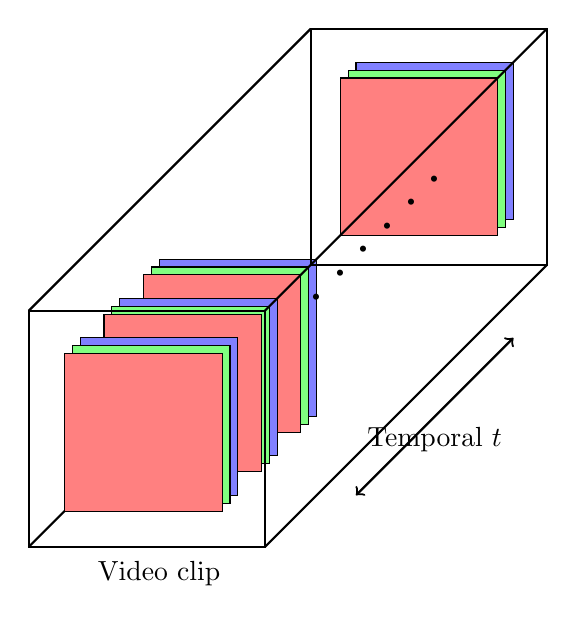
\begin{tikzpicture}
    % 3D Cube - we want to draw some of the cube edges below the frames
    % variables
    \def\cubeWidth{3}
    \def\cubeHeight{3}
    % \def\cubeDepth{8}

    % Cube points
    \coordinate (A) at (0, 0, -5);
    \coordinate (B) at (\cubeWidth, 0, -5);
    \coordinate (C) at (\cubeWidth, \cubeHeight, -5);
    \coordinate (D) at (0, \cubeHeight, -5);
    \coordinate (E) at (-0.5, -0.5, 3);
    \coordinate (F) at (\cubeWidth - 0.5, -0.5, 3);
    \coordinate (G) at (\cubeWidth - 0.5, \cubeHeight - 0.5, 3);
    \coordinate (H) at (-0.5, \cubeHeight - 0.5, 3);

    % Draw cube edges that are below the frames
    \draw[thick] (A) -- (E);

    \def\width{2}
    \def\height{2}
    \def\shift{0.1} % Shift for the green and red channels

    \def\xshift{-0.5}  % Shift in the x direction for duplication
    \def\yshift{-0.5}  % Shift in the y direction for duplication
    \def\lastrectxshift{\xshift * -5} % Last image should be shifted more because of three dots
    \def\lastrectyshift{\yshift * -5} % Last image should be shifted more because of three dots
    \def\dotstartx{2}  % Starting x position for the dots
    \def\dotstarty{1.5}  % Starting y position for the dots
    \def\dotshift{0.3}  % Shift for the dots


    % First rectangle
    \draw[fill=blue!50] (0, 0) rectangle (\width, \height);
    \draw[fill=green!50] (-\shift, -\shift) rectangle (\width-\shift, \height-\shift);
    \draw[fill=red!50] (-2*\shift, -2*\shift) rectangle (\width-2*\shift, \height-2*\shift);

    % Second rectangle
    \draw[fill=blue!50] (\xshift, \yshift) rectangle (\xshift+\width, \yshift+\height);
    \draw[fill=green!50] (\xshift-\shift, \yshift-\shift) rectangle (\xshift+\width-\shift, \yshift+\height-\shift);
    \draw[fill=red!50] (\xshift-2*\shift, \yshift-2*\shift) rectangle (\xshift+\width-2*\shift, \yshift+\height-2*\shift);

    % Third rectangle
    \draw[fill=blue!50] (2*\xshift, 2*\yshift) rectangle (2*\xshift+\width, 2*\yshift+\height);
    \draw[fill=green!50] (2*\xshift-\shift, 2*\yshift-\shift) rectangle (2*\xshift+\width-\shift, 2*\yshift+\height-\shift);
    \draw[fill=red!50] (2*\xshift-2*\shift, 2*\yshift-2*\shift) rectangle (2*\xshift+\width-2*\shift, 2*\yshift+\height-2*\shift);

    % Fourth rectangle
    \draw[fill=blue!50] (\lastrectxshift, \lastrectyshift) rectangle (\lastrectxshift+\width, \lastrectyshift+\height);
    \draw[fill=green!50] (\lastrectxshift-\shift, \lastrectyshift-\shift) rectangle (\lastrectxshift+\width-\shift, \lastrectyshift+\height-\shift);
    \draw[fill=red!50] (\lastrectxshift-2*\shift, \lastrectyshift-2*\shift) rectangle (\lastrectxshift+\width-2*\shift, \lastrectyshift+\height-2*\shift);


    % Dots
    \node at (\dotstartx, \dotstarty) {\huge$\cdot$};
    \node at (\dotstartx + \dotshift, \dotstarty + \dotshift) {\huge$\cdot$};
    \node at (\dotstartx + \dotshift*2, \dotstarty + 2*\dotshift) {\huge$\cdot$};
    \node at (\dotstartx + \dotshift*3, \dotstarty + 3*\dotshift) {\huge$\cdot$};
    \node at (\dotstartx + \dotshift*4, \dotstarty + 4*\dotshift) {\huge$\cdot$};
    \node at (\dotstartx + \dotshift*5, \dotstarty + 5*\dotshift) {\huge$\cdot$};

    % Arrow
    \draw[<->, thick] (2.5, -1) -- (4.5, 1) node[midway, below] {Temporal $t$};







    % Draw the rest of the cube
    \draw[thick] (A) -- (B) -- (C) -- (D) -- cycle;
    \draw[thick] (E) -- (F) -- (G) -- (H) -- cycle;
    \draw[thick] (B) -- (F);
    \draw[thick] (C) -- (G);
    \draw[thick] (D) -- (H);

    % Draw clip text
    \node at (0, -2) {Video clip};

    

\end{tikzpicture}

        }
        \caption{Multiple frames. The $t\ c\ h\ w$ dimensions.}
    \end{subfigure}

    \begin{subfigure}{0.7\textwidth}
        \centering
        \scalebox{0.5}{
            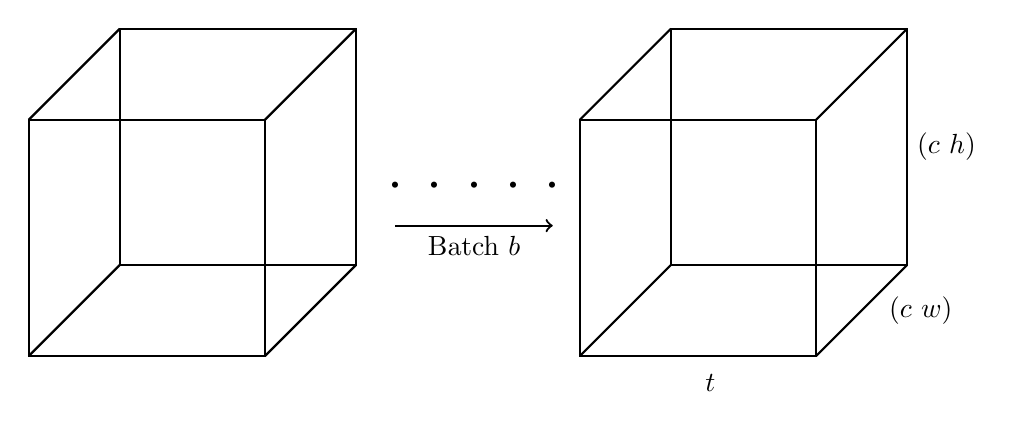
\begin{tikzpicture}
    % First cube
        % variables
        \def\cubeWidth{3}
        \def\cubeHeight{3}
        \def\cubeDepth{3}
    
        % Cube points
        \coordinate (A) at (0, 0, 0);
        \coordinate (B) at (\cubeWidth, 0, 0);
        \coordinate (C) at (\cubeWidth, \cubeHeight, 0);
        \coordinate (D) at (0, \cubeHeight, 0);
        \coordinate (E) at (0, 0, \cubeDepth);
        \coordinate (F) at (\cubeWidth, 0, \cubeDepth);
        \coordinate (G) at (\cubeWidth, \cubeHeight, \cubeDepth);
        \coordinate (H) at (0, \cubeHeight, \cubeDepth);
    
        % Draw cube
        \draw[thick] (A) -- (B) -- (C) -- (D) -- cycle;
        \draw[thick] (E) -- (F) -- (G) -- (H) -- cycle;
        \draw[thick] (A) -- (E);
        \draw[thick] (B) -- (F);
        \draw[thick] (C) -- (G);
        \draw[thick] (D) -- (H);
    
        % Axes
        \node at (0.5, -1.5, 0) {$t$};
        \node at (\cubeWidth + 0.5, \cubeHeight/2, 0) {$(c\ h)$};
        \node at (\cubeWidth + 0.75, 0, \cubeDepth/2) {$(c\ w)$};

    % Second cube
        % variables
        \def\cubeShiftX{-7}
        \def\cubeShiftY{0}
    
        % Cube points (shifted)
        \coordinate (A') at (\cubeShiftX, \cubeShiftY, 0);
        \coordinate (B') at (\cubeShiftX + \cubeWidth, \cubeShiftY, 0);
        \coordinate (C') at (\cubeShiftX + \cubeWidth, \cubeShiftY + \cubeHeight, 0);
        \coordinate (D') at (\cubeShiftX, \cubeShiftY + \cubeHeight, 0);
        \coordinate (E') at (\cubeShiftX, \cubeShiftY, \cubeDepth);
        \coordinate (F') at (\cubeShiftX + \cubeWidth, \cubeShiftY, \cubeDepth);
        \coordinate (G') at (\cubeShiftX + \cubeWidth, \cubeShiftY + \cubeHeight, \cubeDepth);
        \coordinate (H') at (\cubeShiftX, \cubeShiftY + \cubeHeight, \cubeDepth);
    
        % Draw the second cube
        \draw[thick] (A') -- (B') -- (C') -- (D') -- cycle;
        \draw[thick] (E') -- (F') -- (G') -- (H') -- cycle;
        \draw[thick] (A') -- (E');
        \draw[thick] (B') -- (F');
        \draw[thick] (C') -- (G');
        \draw[thick] (D') -- (H');

    % Three dots
        % variables
        \def\dotStartX{-3.5}
        \def\dotStartY{1}
        \def\dotShiftX{0.5}
        \def\dotShiftY{0}
    
        % dots
        \node at (\dotStartX, \dotStartY) {\huge$\cdot$};
        \node at (\dotStartX + \dotShiftX, \dotStartY + \dotShiftY) {\huge$\cdot$};
        \node at (\dotStartX + \dotShiftX * 2, \dotStartY + \dotShiftY * 2) {\huge$\cdot$};
        \node at (\dotStartX + \dotShiftX * 3, \dotStartY + \dotShiftY * 3) {\huge$\cdot$};
        \node at (\dotStartX + \dotShiftX * 4, \dotStartY + \dotShiftY * 4) {\huge$\cdot$};


    % Arrow
    \draw[->, thick] (-3.5, 0.5) -- (-1.5, 0.5) node[midway, below] {Batch $b$};
\end{tikzpicture}
        }
        \caption{All the $b\ t\ c\ h\ w$ dimensions.}
    \end{subfigure}

    \caption{Representation of video dimensions $b\ t\ c\ h\ w$ which corresponds to batch, temporal, channel, height, width dimensions.}
\end{figure}





\textbf{Mixing factor}: after each temporal layer, the output $z'$ is combined with the output of previous spatial layer output $z$ to form a mixing: 

\[ \underbrace{\alpha_\phi^i z_{i} + (1 - \alpha_\phi^i) z_{i}'}_{\text{Mixing factor}} \] 

where $\alpha_\phi^i \in [0, 1]$ and is a learnable parameter. If we set $\alpha = 1$ for each layer skip the temporal score, and we retain the native image generation capability. This mixing operation is similar to CFG (mixing between conditional score and unconditional score).

\textbf{Temporal mixing layers}: two types of temporal mixing layers in use (see figure \ref{fig:video_ldm_spatial_temporal_mixing_layers}) are the \textit{temporal attention} and \textit{Conv3D} layer.

\textbf{Noise scheduler}: Video-LDM uses the same noise scheduler as the underlying image model. In table 6 of the paper, it shows that in all of their models, they use linear noise scheduler.

\textbf{Training objective}: in the training phase only the temporal layers are trained. The objective is the LDM objective (likelihood based, predicting noise in U-Net):

\[ \arg \min_\phi \mathbb{E}_{x \sim p_{\text{data}}, \tau \sim p_{\tau}, \epsilon \sim \mathcal{N} (0, I)} \left[ \left| \left| y - f_{\theta,\phi} (z_{\tau} ; c, \tau) \right| \right|^2_2 \right] \]

where $\tau$ is the diffusion time step, $y$ is the target noise vector. The target is to minimize the difference between predicted noise and ground truth $y$ over all video frames.

\textbf{Adding temporal layers to the decoder:} the researchers add temporal layers to the decoder of the AE which they found this step to be critical for achieving good results. The reason is that the AE is trained on images and flickering artifacts are present in the generated videos (because training on images doesn't teach the model temporal dynamics). So the researchers fine-tune the decoder on video data with a \textbf{patch-wise temporal discriminator built from 3D convolutions}. The encoder, however, remains unchanged.

\textbf{Patch-wise temporal discriminator:} The patch-wise temporal discriminator $\mathcal{H}$, which is built from 3D convolutions, is used to fine-tune the decoder. It is trained on video data and returns "real" or "fake" prediction on patches of the video clip.


\begin{figure}
    \centering
    \scalebox{0.4}{
        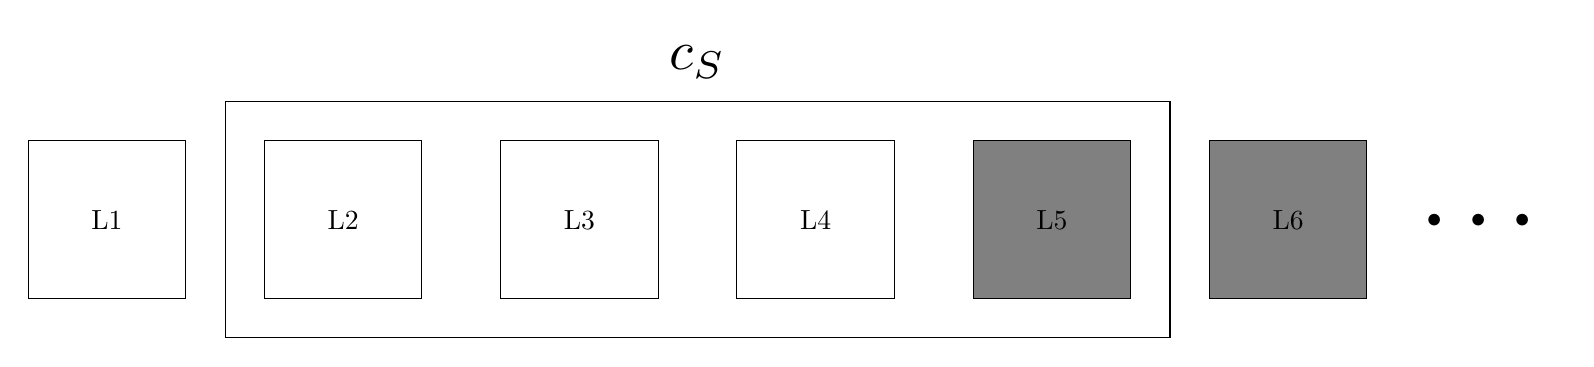
\begin{tikzpicture}
    \draw[fill=white!50] (0, 0) rectangle (2, 2);
    \node[anchor=center] at (1, 1) {L1};

    \draw[fill=white!50] (3, 0) rectangle (5, 2);
    \node[anchor=center] at (4, 1) {L2};

    \draw[fill=white!50] (6, 0) rectangle (8, 2);
    \node[anchor=center] at (7, 1) {L3};

    \draw[fill=white!50] (9, 0) rectangle (11, 2);
    \node[anchor=center] at (10, 1) {L4};

    \draw[fill=black!50] (12, 0) rectangle (14, 2);
    \node[anchor=center] at (13, 1) {L5};

    \draw[fill=black!50] (15, 0) rectangle (17, 2);
    \node[anchor=center] at (16, 1) {L6};

    % c_S
    \node[anchor=center, scale=2] at (8.5,3) {$c_S$};

    % Context guidance box
    \draw[] (2.5, -0.5) rectangle (14.5, 2.5);

    % 3 Dots
    \node [scale=4] at (18,1) {\rotatebox{90}{$\vdots$}};
\end{tikzpicture}
    }
    \caption{Keyframe model learns to predict the next latent frame $z$ by context guidance (conditioned on previous frames).}
\end{figure}

\begin{figure}
    \centering
    \scalebox{0.4}{
        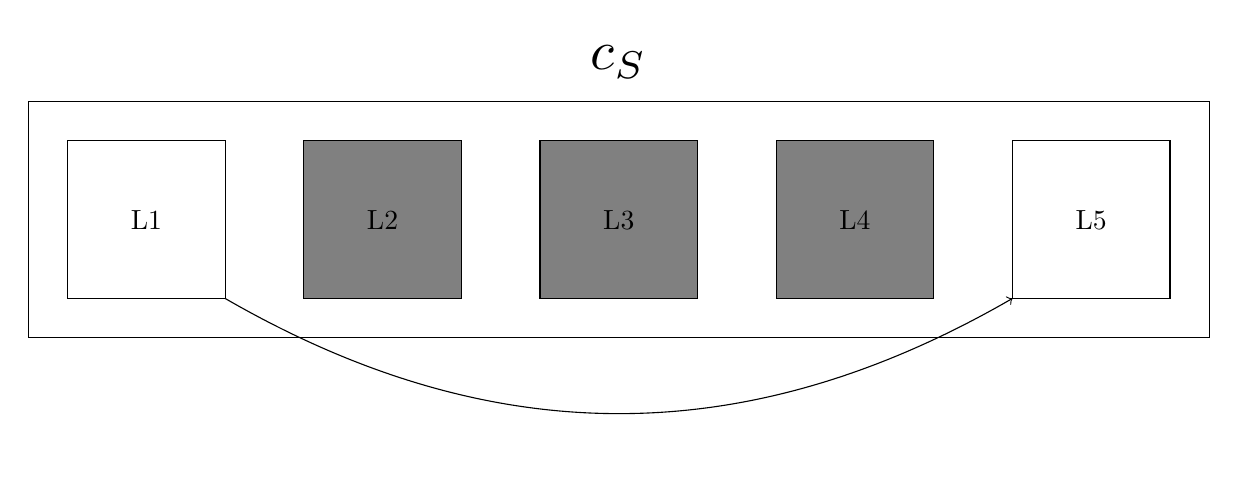
\begin{tikzpicture}
    \draw[fill=white!50] (0, 0) rectangle (2, 2);
    \node[anchor=center] at (1, 1) {L1};

    \draw[fill=black!50] (3, 0) rectangle (5, 2);
    \node[anchor=center] at (4, 1) {L2};

    \draw[fill=black!50] (6, 0) rectangle (8, 2);
    \node[anchor=center] at (7, 1) {L3};

    \draw[fill=black!50] (9, 0) rectangle (11, 2);
    \node[anchor=center] at (10, 1) {L4};

    \draw[fill=white!50] (12, 0) rectangle (14, 2);
    \node[anchor=center] at (13, 1) {L5};

    \draw[->] (2, 0) to[bend right] (12, 0);

    \node[anchor=center, scale=2] at (7,3) {$c_S$};
    \draw[] (-0.5, -0.5) rectangle (14.5, 2.5);
\end{tikzpicture}
    }
    \caption{Interpolation model learns to fill masked latents $m \circ z$ (L2, L3, L4) in between two keyframes latents (L1, L5) with context guidance.}
\end{figure}

\textbf{Context guidance \& Masking}: the model can be conditioned on context information, and is denoted with $c_S$ in figure \ref{fig:video_ldm_spatial_temporal_mixing_layers}. The model is conditioned on the initial set of $S$ context frames, which are the frames at the beginning of the clip. A temporal binary mask is applied to the frames that the model must predict, so the model knows which frames it must predict and which are the context. The latent vector generated by the encoder is concatenated with the binary mask, forming the context guidance $c_S$.

\textbf{Temporal binary mask \& Higher FPS}: in order to adapt to long duration videos, the researchers trained a $T \rightarrow 4T$ keyframe interpolation model, where for each two keyframes, the model interpolate between them and generates 3 additional frames by using binary masks $m_S$ (0 or 1). The frames are multiplied by the mask and the model learns to predict the missing (masked) frames. This technique achieves higher FPS.

\textbf{LDM Decoder}: the latents are then decoded to the pixel space using the LDM decoder.

\textbf{Upsampler (L)DM}: to increase the spatial resolution of generated frames, they used a SR model, inspired by cascaded DMs \cite{cascaded_diffusion_models} (the SR3 model \cite{sr3}). In their experiments they used \textbf{pixel-space DM upsampler}, whereas for T2V models they used \textbf{LDM upsampler}. Since upsampling video frames independently would result in poor temporal consistency, they made the SR model video-aware by adding temporal layers and mixing spatial and temporal layers, in similar manner as discussed before.

\textbf{Number of parameters}: the Video-LDM model (except for the CLIP text encoder) consists of 3.1 billion parameters (AE and diffusion models [keyframe generation model, interpolation model, upsamplers]), and only 2.2 billion of these parameters are actually trained:

\begin{itemize}
    \item 84 million parameters in the AE
    \item 865 million parameters in the image backbone LDM, not including CLIP text encoder
    \item 655 million parameters in temporal layers
    \item 354 million parameters in the text encoder (OpenCLIP-ViT/H)
    \item 1.5 million parameters in the interpolation latent diffusion model
\end{itemize}

Compared to Imagen (11.6 billion parameters) and CogVideo (9 billion parameters), Video-LDM is much smaller yet produced high quality videos partly because it works in latent space.

\textbf{DDIM Sampling}: in appendix F of the paper they write that they use the DDIM sampler \cite{ddim} (section \ref{subsec:ddim_sampler}), where the stochastically $\eta$ is varied, as well as the guidance scale.

\textbf{CLIP text encoder}: the text encoder (for T2V conditioning) is a CLIP \cite{openai_clip} based model which is used to generate text embeddings, as we discussed before (section \ref{subsec:clip}).










\subsection{Experiments}

\begin{figure}
    \centering
    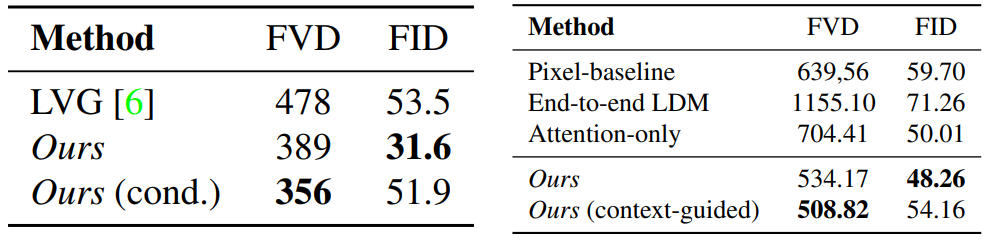
\includegraphics[width=0.5\textwidth]{images/video_ldm/videoldm_vs_lvg_on_rds.png}
    \caption{Comparison of Video-LDM and Long Video GAN (LVG) on RDS dataset \cite{video_ldm}.}
    \label{fig:video_ldm_vs_lvg_on_rds}
\end{figure}

In figure \ref{fig:video_ldm_vs_lvg_on_rds} we see comparison of Video-LDM and Long Video GAN (LVG) on RDS dataset. \texttt{Cond.} means the model was conditioned on day/night and crowdedness\footnote{In their experiments, they observed that adding conditional information reduces FID and FVD metrics.}. On the right we see FVD and FID evaluations on different diffusion architectures (pixel-space diffusion model, end-to-end LDM that was not pre-trained on images [which is why the results are bad], and attention-only temporal model). Their model uses 3D temporal convolutions which is better than the attention-only diffusion model.

\begin{figure}
    \centering
    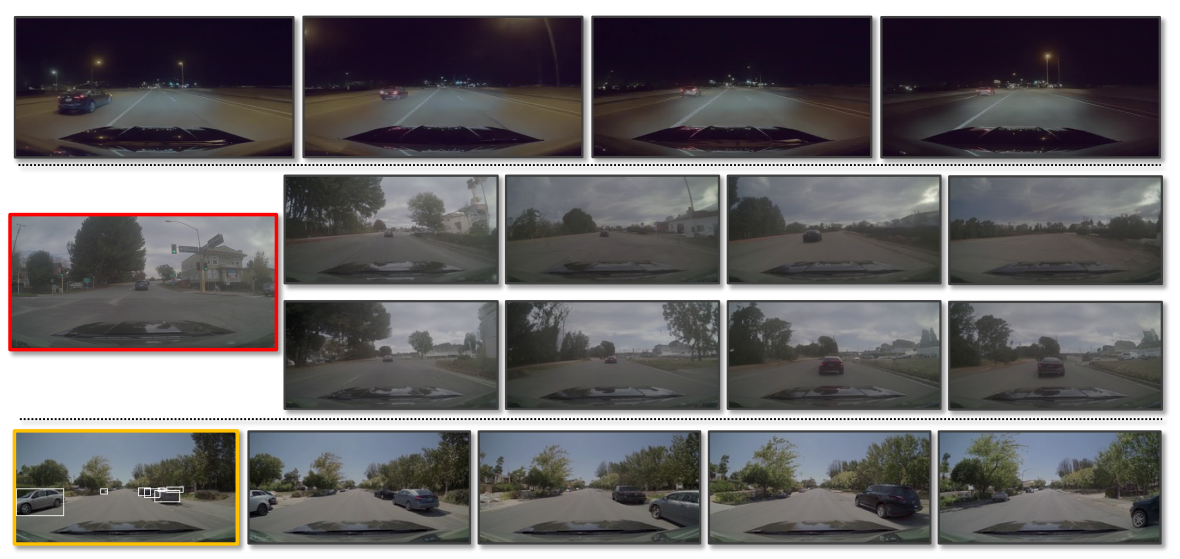
\includegraphics[width=0.5\textwidth]{images/video_ldm/rds.png}
    \caption{Real driving videos (RDS) generation samples \cite{video_ldm}.}
    \label{fig:video_ldm_rds}
\end{figure}

In figure \ref{fig:video_ldm_rds} we see real driving videos (RDS) samples. \textit{Top}: night videos. \textit{Middle}: the left red frame is the condition input, while the right is two different generated samples (given a frame, the model can generate the next frames). \textit{Bottom}: they trained a separate bounding-box conditioned LDM for image synthesis only (the RDS dataset has some bounding-box clips), which generates initial frame (in yellow), and then Video-LDM completes the video generation based on this frame.

\begin{figure}
    \centering
    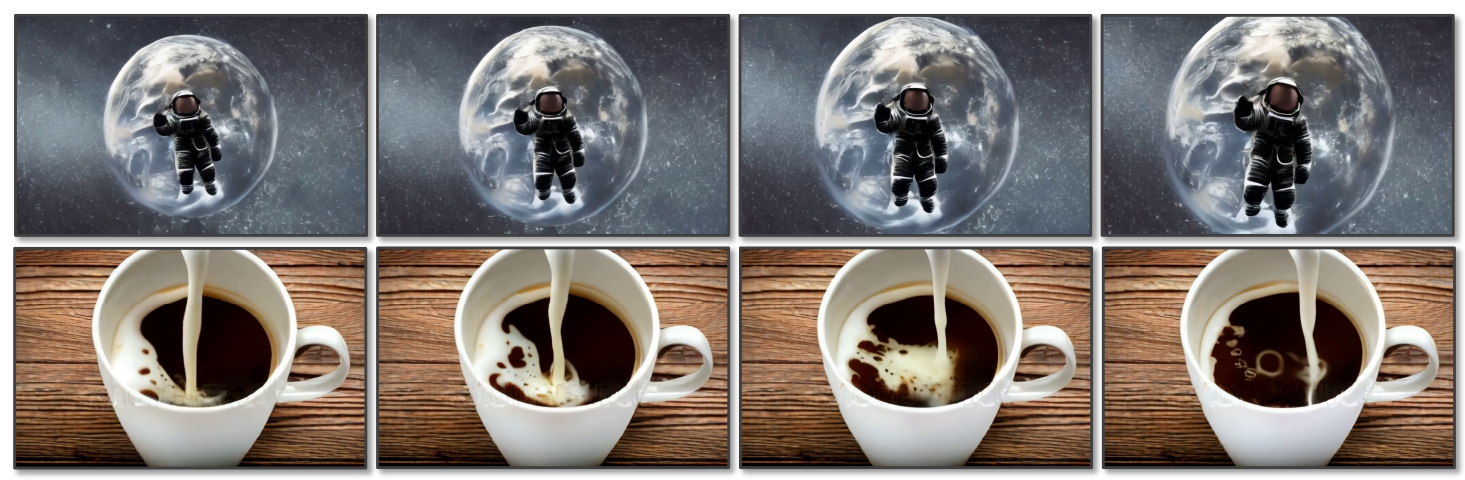
\includegraphics[width=0.5\textwidth]{images/video_ldm/webvid_samples.png}
    \caption{Generated samples trained on WebVid-10M dataset. Prompts: "An astronaut flying in space, 4k, high resolution" and "Milk dripping into a cup of coffee, high definition, 4k" \cite{video_ldm}.}
    \label{fig:video_ldm_webvid_samples}
\end{figure}

We can see text conditioned samples in figure \ref{fig:video_ldm_webvid_samples} on the WebVid-10M dataset at $1280\times 2048$ resolution.

\begin{figure}
    \centering

    \begin{subfigure}{0.8\textwidth}
        \centering
        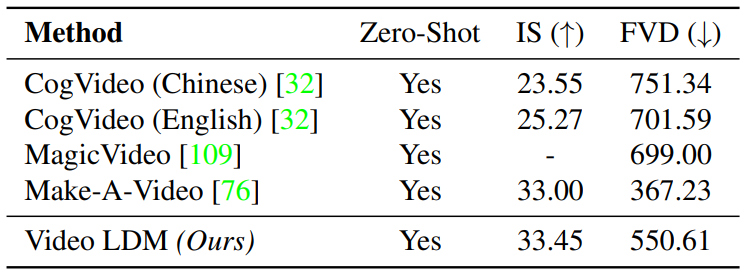
\includegraphics[width=0.5\textwidth]{images/video_ldm/ucf.png}
        \caption{UCF-101 dataset. Video-LDM achieves the best inception score.}
    \end{subfigure}

    \begin{subfigure}{0.8\textwidth}
        \centering
        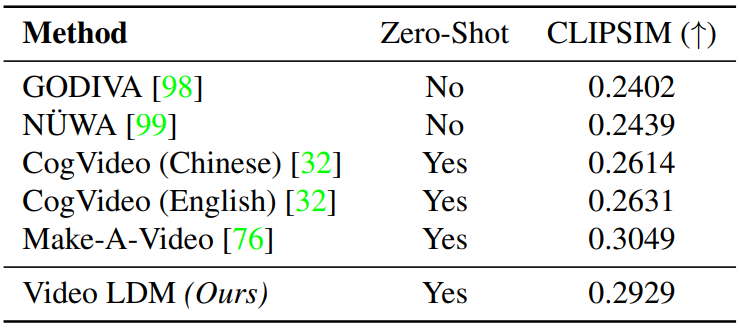
\includegraphics[width=0.5\textwidth]{images/video_ldm/msr_vtt.png}
        \caption{MSR-VTT dataset. Video-LDM almost achieves the best CLIP-SIM score.}
    \end{subfigure}

    \caption{Video-LDM is compared to other state-of-the-art models in zero-shot setting on UCF-101 and MSR-VTT datasets \cite{video_ldm}.}
\end{figure}

The researchers used the following datasets:

\begin{itemize}
    \item \textbf{RDS (Real Driving Videos)}: An in-house dataset of 683,060 videos (up to 8 seconds @ $512\times 1024$ @ 30 fps) with day/night labels and "crowdedness" annotations. Some include car bounding boxes. They used label dropout for CFG and compared Video-LDM to Long Video GAN (LVG) on this dataset (figure \ref{fig:video_ldm_vs_lvg_on_rds}).
    \item \textbf{WebVid-10M}: Contains 10.7M video-caption pairs (52K hours total). They fine-tuned Stable Diffusion spatial layers on frames, added temporal layers, and trained with captions. Upsampled videos to $1280\times 2048$ resolution. Samples are 113 frames (4.7s @ 24 fps or 3.8s @ 30 fps).
    \item \textbf{Mountain Bike Dataset} \cite{brooks2022generating}: Introduced by LVG, it contains 1,202 clips ($\geq 5$ seconds @ 30 fps).
\end{itemize}

\textbf{Evaluation metrics}: they used FID to evaluate quality of individual frames. They also used FVD and human evaluation on video clips and compared to LVG. The human evaluation contained 100 videos @ 4 seconds; given a pair of videos (one from Video-LDM and one from LVG), participants select the most favorable.

\textbf{Video synthesis on RDS dataset}: for video synthesis on RDS dataset, they first generate a single frame using the image LDM, then they run the prediction model on a single frame and generated a sequence of keyframes. Next they performed two steps of the interpolation model which increases the FPS from 1.875 to 7.5 and from 7.5 to 30 fps. And then they ran the temporal upsampler which is run over portions of 8 video frames (the upsampler is also temporally aligned). In their experiments, the researchers successfully generated long, temporally coherent, high-resolution driving videos (up to 5 minutes), trained on the RDS dataset.

